
% This LaTeX was auto-generated from an M-file by MATLAB.
% To make changes, update the M-file and republish this document.

%%% \documentclass{article}
%%% \usepackage{graphicx}
%%% \usepackage{color}

%%% \sloppy
%%% \definecolor{lightgray}{gray}{0.5}
\setlength{\parindent}{0pt}

%%% \begin{document}

    
    
\subsection*{Simple example of the QWTB use}

\begin{par}
Sample data are simulated. QWTB is used to apply two different algorithms on the same data. Uncertainty of the results is calculated by means of Monte Carlo Method.
\end{par} \vspace{1em}

\subsubsection*{Contents}

\begin{itemize}
\setlength{\itemsep}{-1ex}
   \item Generate sample data
   \item Analyzing data
   \item Uncertainties
\end{itemize}


\subsubsection*{Generate sample data}

\begin{par}
Two quantities are prepared: \lstinline{t} and \lstinline{y}, representing 0.5 second of sinus waveform of nominal frequency 1 kHz, nominal amplitude 1 V and nominal phase 1 rad, sampled at sampling frequency \lstinline{fsnom} 10 kHz.
\end{par} \vspace{1em}
\begin{lstlisting}[style=mcode]
DI = [];
Anom = 1; fnom = 1e3; phnom = 1; fsnom = 1e4;
DI.t.v = [0:1/fsnom:0.5];
DI.y.v = Anom*sin(2*pi*fnom*DI.t.v + phnom);
\end{lstlisting}
\begin{par}
Add noise of standard deviation 1 mV:
\end{par} \vspace{1em}
\begin{lstlisting}[style=mcode]
DI.y.v = DI.y.v + normrnd(0, 1e-3, size(DI.y.v));
\end{lstlisting}


\subsubsection*{Analyzing data}

\begin{par}
To get a frequency spectrum, algorithm \lstinline{SP-FFT} can be used. This algorithm requires sampling frequency, so third quantity \lstinline{fs} is added.
\end{par} \vspace{1em}
\begin{lstlisting}[style=mcode]
DI.fs.v = fsnom;
DO = qwtb('SP-FFT', DI);
plot(DO.f.v, DO.A.v, '-xb'); xlim([980 1020])
\end{lstlisting}

        \begin{lstlisting}[style=output]
QWTB: no uncertainty calculation
Warning: Integer operands are required for colon operator when used as index 
\end{lstlisting} \color{black}
    
\begin{center}
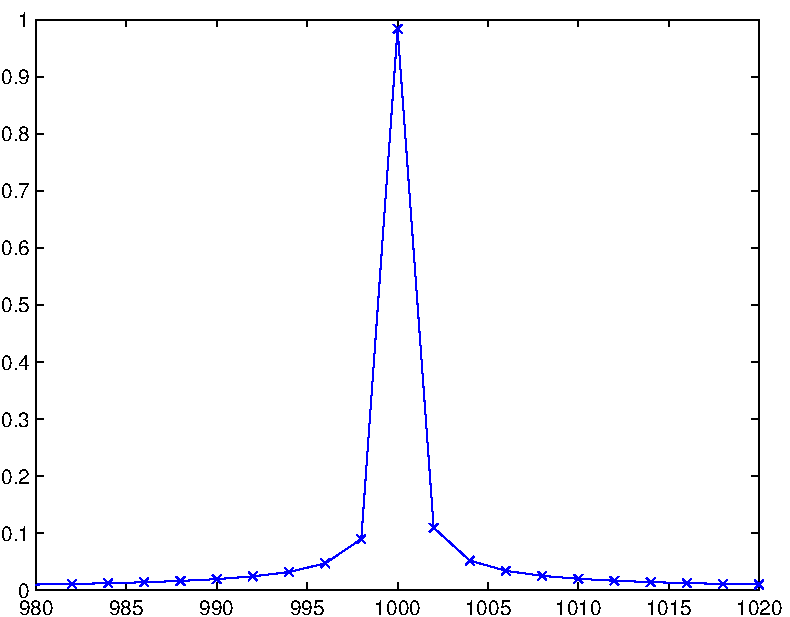
\includegraphics[width=0.7\textwidth]{qwtb_examples_published/qwtb_example_1_01.pdf}
\end{center}
\begin{par}
One can see it is not a coherent measurement. Therefore to get 'unknown' amplitude and frequency of the signal algorithm \lstinline{PSFE} can be used:
\end{par} \vspace{1em}
\begin{lstlisting}[style=mcode]
DO = qwtb('PSFE', DI);
f = DO.f.v
A = DO.A.v
\end{lstlisting}

        \begin{lstlisting}[style=output]
QWTB: no uncertainty calculation

f =

   1.0000e+03


A =

    1.0000

\end{lstlisting} \color{black}
    

\subsubsection*{Uncertainties}

\begin{par}
Uncertainties are added to the \lstinline{t} (time stamps) and \lstinline{y} (sampled data) structures.
\end{par} \vspace{1em}
\begin{lstlisting}[style=mcode]
DI.t.u = zeros(size(DI.t.v)) + 1e-5;
DI.y.u = zeros(size(DI.y.v)) + 1e-4;
\end{lstlisting}
\begin{par}
Calculations settings is created with Monte Carlo uncertainty calculation method, 1000 repeats and singlecore calculation.
\end{par} \vspace{1em}
\begin{lstlisting}[style=mcode]
CS.unc = 'mcm';
CS.mcm.repeats = 1000;
CS.mcm.method = 'singlecore';
\end{lstlisting}
\begin{par}
Run PSFE algorithm on input data \lstinline{DI} and with calculattion settings \lstinline{CS}.
\end{par} \vspace{1em}
\begin{lstlisting}[style=mcode]
DO = qwtb('PSFE',DI,CS);
\end{lstlisting}

        \begin{lstlisting}[style=output]
QWTB: default correlation matrix generated for quantity `t`
QWTB: quantity t was randomized by QWTB
QWTB: default correlation matrix generated for quantity `y`
QWTB: quantity y was randomized by QWTB
QWTB: general mcm uncertainty calculation
\end{lstlisting} \color{black}
    \begin{par}
Result is displayed as a histogram of calculated frequency.
\end{par} \vspace{1em}
\begin{lstlisting}[style=mcode]
figure; hist(DO.f.r,50);
\end{lstlisting}

\begin{center}
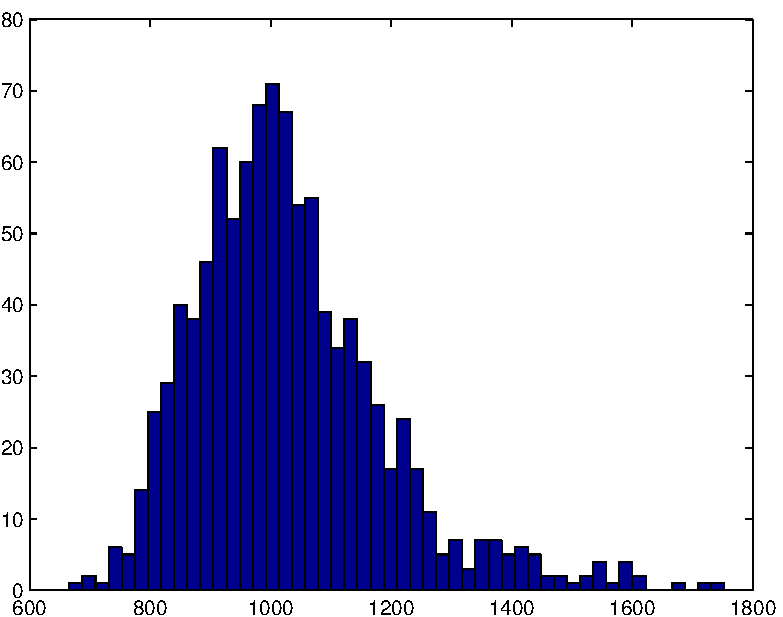
\includegraphics[width=0.7\textwidth]{qwtb_examples_published/qwtb_example_1_02.pdf}
\end{center}
\begin{par}
One can see the histogram is not Gaussian function. To get correct uncertainties, a shortest covariant interval has to be used.
\end{par} \vspace{1em}



%%% \end{document}
    
